\anothertitle{Conclusion and Future Work}{}

% Two-column with image 
\begin{frame}
  \Frametitle{Conclusion}

  \begin{columns}
    \column{0.4\textwidth}
      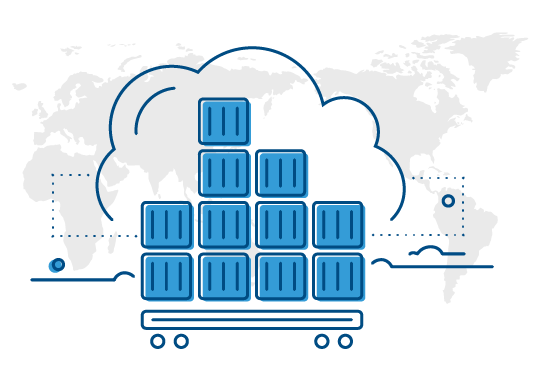
\includegraphics[keepaspectratio,width=\textwidth,height=\textheight]{cloudContainer}  
  
    \column{0.6\textwidth}
      \bullettext{This project aimed to compare \emph{Cloud Container Orchestration} platforms in respect to}:
      \begin{itemize}
            \item \bullettext{ease of adoption and configuration}
            \item \bullettext{deployment process}
            \item \bullettext{restrictions and limitations}
            \item \bullettext{performance}
            \item \bullettext{cost impacts}
            \item \bullettext{reliability and resilience}
      \end{itemize}

    \end{columns}
  
\end{frame}

\begin{frame}
  \Frametitle{Concluding Statements}
  
  \begin{itemize}
        \item \bullettext{Selection of container-orchestration \textbf{platform} will have a \textbf{minor} impact on \textit{performance}}
        \item \bullettext{Selection of underlying \textbf{server-architecture} has a far more \textbf{significant} impact on \textit{performance}}
        \item \bullettext{\textbf{Network latency} does not mask the potential \textbf{loss} in (measurable) \textit{performance} }
        \item \bullettext{Limitations of \textbf{Serverless Functions} results in the technology being an inviable choice as a container orchestration platform}
        \item \bullettext{\textbf{Cloud-Native} container orchestration platforms provide a more \textbf{consistent} cloud experience at the cost of \textbf{performance} and vendor \textbf{lock-in} }
        \item \bullettext{Managed Cloud \textbf{Kubernetes} platforms benefit from their \textbf{open-source} architecture (in terms of \textit{support} and \textit{performance}) at the cost of \textbf{complexity} and \textbf{monetary costing}}
  \end{itemize}
  
\end{frame}

\begin{frame}
  \Frametitle{Future Work}

  \begin{columns}
    \column{0.6\textwidth}
      \begin{itemize}
            \item \bullettext{Comparison in terms of \textit{adoption} vs \textit{migration}}
            \item \bullettext{Verification of cloud vendors' claim of feature-parity with AWS}
            \item \bullettext{Creating benchmark suites which specficially cater for Serverless Function }
      \end{itemize}

    \column{0.4\textwidth}
      
\includegraphics[keepaspectratio,width=\textwidth,height=\textheight]{cloudContainerOnSea}  
  
  \end{columns}
  
\end{frame}